%!TEX root=../document.tex

\section{Ergebnisse}

\subsection{Eine Klasse erbt von Thread}

\begin{lstlisting}[language=python]
import threading
class A06(threading.Thread):
\end{lstlisting}

\subsection{Gemeinsamer Lock und Counter}
\begin{lstlisting}[language=python]
counter = 0
lock = threading.Lock()
\end{lstlisting}

\subsection{Paramter im Konstruktor}

\begin{lstlisting}[language=python]
    def __init__(self, tNumbers):
        """

        :param tNumbers: Eine Liste aus Nummern welche der jweilige Thread zo counter dazu addieren soll
        """
\end{lstlisting}

\subsection{Korrekt aufsummieren}

\begin{lstlisting}[language=python]
    def run(self):
        for i in range(len(self.tNumbers)):
            with A06.lock:
                # hier wird counter immer um die Zahl an der Stellle 0 der liste erhoeht
                # dann wird die Stelle 0 geloescht und alles rueckt nach links(2 -> 1, 1 -> 0, etc.)
                A06.counter += self.tNumbers[0]
                print("Current Value: " + str(A06.counter))
                del(self.tNumbers[0])
\end{lstlisting}
\clearpage
\subsection{Der ganze Code}

\begin{lstlisting}[language=python]
import threading
import time

class A06(threading.Thread):
    # globale Variable counter welche von jedem Thread benutzt wird
    counter = 0
    lock = threading.Lock()
    def __init__(self, tNumbers):
        """

        :param tNumbers: Eine Liste aus Nummern welche der jweilige Thread zo counter dazu addieren soll
        """
        threading.Thread.__init__(self)
        self.tNumbers = tNumbers
    def run(self):
        for i in range(len(self.tNumbers)):
            with A06.lock:
                # hier wird counter immer um die Zahl an der Stellle 0 der liste erhoeht
                # dann wird die Stelle 0 geloescht und alles rueckt nach links(2 -> 1, 1 -> 0, etc.)
                A06.counter += self.tNumbers[0]
                print("Current Value: " + str(A06.counter))
                del(self.tNumbers[0])

def getInput():
    """

    :return: Die eingabe
    """
    # Die eingabe gleich als int
    n = int(input("Bitte geben sie die Zahl ein bis zu der addiert werden soll."))
    return n

def main1Threads(numberHelp):
    """

    :param numberHelp: die eingabe
    """
    anfang = time.time()#Anfang des Programms
    # numberHelp = getInput()

    # Die Listen fuer die Threads
    tN1 = []
    for i in range(1, numberHelp + 1):
        tN1.append(i)

    # Die Threads + start() und join()
    t = A06(tN1)

    t.start()

    t.join()

    lz = time.time() - anfang#Die ausgerechnete Laufzeit, Ende - Anfang
    print("mit 1 Threads: " + str(lz))

def main2Threads(numberHelp):
    """

    :param numberHelp: die eingabe
    """
    anfang = time.time()#Anfang des Programms
    # numberHelp = getInput()

    #Die Listen fuer die Threads
    tN1 = []
    tN2 = []
    for i in range(1, numberHelp + 1, 2):
        tN1.append(i)
    for i in range(2, numberHelp + 1, 2):
        tN2.append(i)

    #Die Threads + start() und join()
    t = A06(tN1)
    t2 = A06(tN2)

    t.start()
    t2.start()

    t.join()
    t2.join()

    lz = time.time() - anfang#Die ausgerechnete Laufzeit, Ende - Anfang
    print("mit 2 Threads: " + str(lz))

def main3Threads(numberHelp):
    """

    :param numberHelp: die eingabe
    """
    anfang = time.time()#Anfang des Programms
    #numberHelp = getInput()

    # Die Listen fuer die Threads
    tN1 = []
    tN2 = []
    tN3 = []
    for i in range(1,numberHelp+1,3):
        tN1.append(i)
    for i in range(2,numberHelp+1,3):
        tN2.append(i)
    for i in range(3,numberHelp+1,3):
        tN3.append(i)

    # Die Threads + start() und join()
    t = A06(tN1)
    t2 = A06(tN2)
    t3 = A06(tN3)

    t.start()
    t2.start()
    t3.start()

    t.join()
    t2.join()
    t3.join()

    lz = time.time() - anfang#Die ausgerechnete Laufzeit, Ende - Anfang
    print("mit 3 Threads: " + str(lz))

def main4Threads(numberHelp):
    """

    :param numberHelp: die eingabe
    """
    anfang = time.time()#Anfang des Programms
    #numberHelp = getInput()

    # Die Listen fuer die Threads
    tN1 = []
    tN2 = []
    tN3 = []
    tN4 = []
    for i in range(1,numberHelp+1,4):
        tN1.append(i)
    for i in range(2,numberHelp+1,4):
        tN2.append(i)
    for i in range(3,numberHelp+1,4):
        tN3.append(i)
    for i in range(3, numberHelp + 1, 4):
        tN4.append(i)

    # Die Threads + start() und join()
    t = A06(tN1)
    t2 = A06(tN2)
    t3 = A06(tN3)
    t4 = A06(tN4)

    t.start()
    t2.start()
    t3.start()
    t4.start()

    t.join()
    t2.join()
    t3.join()
    t4.join()


    lz = time.time() - anfang#Die ausgerechnete Laufzeit, Ende - Anfang
    print("mit 4 Threads: " + str(lz))

def main():
    #hier rufe ich die einzehlnen Methoden auf und dazwischen muss ich
    #counter auf 0 setzen da es sich um ein Globale Variable handelt
    numberHelp = getInput()
    main1Threads(numberHelp)
    A06.counter = 0
    main2Threads(numberHelp)
    A06.counter = 0
    main3Threads(numberHelp)
    A06.counter = 0
    main4Threads(numberHelp)

main()
\end{lstlisting}

\subsection{Consol Outpu bei Eingabe 1000}
\begin{figure}[!h]
	\begin{center}
		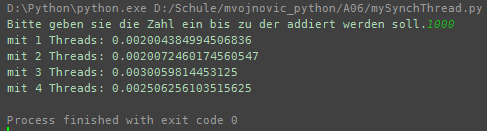
\includegraphics[width=0.7\linewidth]{images/consolOutput.png}
		\caption{Consolen Output}
		\label{broker}
	\end{center}
\end{figure}

\section{Interpretation}

Es ist erkennbar bei wiederholten Versuchen das die Erhoeung der Thread-Anzahl zur verlangsamung des Programmes fuehrt

\section{Massnahmen}

So wenige Threads wie moeglich verwenden